\documentclass[dvipdfmx]{jarticle}
\pagestyle{empty}
\hoffset=-25mm \voffset=-25mm
\setlength{\textwidth}{16cm}
\setlength{\textheight}{24cm}
\usepackage{url}
\usepackage{tikz}
\usetikzlibrary{calc,shapes}
\usepackage{fancyvrb}
\usepackage{tabularx}
\usepackage{multirow}
\newcounter{coffee}
\newcounter{bean}
%\input{mymacros}
\begin{document}
\begin{flushright}
\verb|2026/10/23|
\end{flushright}
\begin{center}{\bf\Large
  2026年度　コンパイラ演習課題(4)[修正版]
}\end{center}
\begin{itemize}
  \item TACTの課題の添付ファイルとしてPDFファイルで提出すること．
  \item 手書きレポートをPDFとして提出する方法は講義webサイトを
  参照\footnote{\url{https://sites.google.com/sqlab.jp/26compiler/how-to-make-report}}すること．
  \item 提出期限: 10月30日(金) 23:55(JST)
\end{itemize}

\begin{list}{{\bf [\,\arabic{coffee}\,]}}{\usecounter{coffee}}
  \item 次のプログラムを目的コードへ変換する際の，プログラムの 1 行目終わり，3 行目
  終わり，8 行目終わりの時点での記号表をそれぞれ示せ．ただし，関数\texttt{exp}の実行コードの開
  始位置は$a_{\texttt{exp}}$とする．

  \begin{Verbatim}[numbers=left]
int x,y,z;
int exp(int x,int y) {
  int rv;
  if (y==0) {rv=1;}
  else if (y<0) {rv=exp(x,y+1)/x;}
  else {rv=x*exp(x,y-1);}
  return rv;
}

main() {
  x=2; z=7; y=exp(x,z);
  printf("%d\n",y);
}
  \end{Verbatim}
\item 各変数に割り当てられている値を以下のものとする．
\begin{center}
	\begin{tabularx}{.75\linewidth}{|X|X||X|X||X|X||X|X|}\hline
		\texttt{x} & $1$ & \texttt{y} & $2$ & \texttt{z} & $3$ & \texttt{w} & $4$\\\hline
	\end{tabularx}
\end{center}
\begin{list}{(\arabic{coffee}-\arabic{bean})}{\usecounter{bean}}
  \item
このとき，以下の逆ポーランド記法の命令が実行されたとき，スタックトップに残る値を求めよ．

\begin{center}
	\begin{tabular}{llcllcp{15zw}}
		\texttt{push} & \texttt{x} & \hspace*{5zw} & \texttt{push} & \texttt{x} & \quad & \multirow{7}{*}{
      \parbox{15zw}{\texttt{add},\texttt{mult}はそれぞれスタックの上から２つの値をpopして
    加算および乗算してその値をスタックトップにpushする．}}\\
		\texttt{push} & \texttt{y} & & \texttt{push} & \texttt{y}\\
		\texttt{add} & & & \texttt{mult} & \\
		\texttt{push} & \texttt{z} & & \texttt{push} & \texttt{z}\\
		\texttt{push} & \texttt{w} & & \texttt{add} & \\
		\texttt{mult} & & & \texttt{push} & \texttt{w}\\
		\texttt{add} & & & \texttt{mult} & \\[3pt]
		\multicolumn{2}{c}{(a)} & & \multicolumn{2}{c}{(b)}\\
	\end{tabular}
\end{center}

\item 以下の抽象構文木として計算される値を求めよ．
\begin{center}
  \begin{tabular}{ccc}
    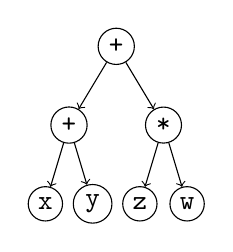
\begin{tikzpicture}
      \node[draw,circle,inner sep=2pt] (M0) at (0,0) {\texttt{+}};
      \node[draw,circle,inner sep=2pt] (M1) at (-0.6,-1) {\texttt{+}};
      \node[draw,circle,inner sep=2pt] (M2) at (0.6,-1) {\texttt{*}};
      \node[draw,circle,inner sep=2pt] (M3) at (-0.9,-2) {\texttt{x}};
      \node[draw,circle,inner sep=2pt] (M4) at (-0.3,-2) {\texttt{y}};
      \node[draw,circle,inner sep=2pt] (M5) at (0.3,-2) {\texttt{z}};
      \node[draw,circle,inner sep=2pt] (M6) at (0.9,-2) {\texttt{w}};
      \path[->] (M0) edge (M1) (M0) edge (M2);
      \path[->] (M1) edge (M3) (M1) edge (M4) (M2) edge (M5) (M2) edge (M6);
    \end{tikzpicture}
    & &
    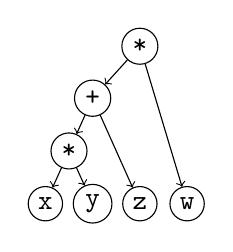
\begin{tikzpicture}
      \node[draw,circle,inner sep=2pt] (N0) at (0,0) {\texttt{*}};
      \node[draw,circle,inner sep=2pt] (N1) at (-0.6,-0.66) {\texttt{+}};
      \node[draw,circle,inner sep=2pt] (N2) at (-0.9,-1.33) {\texttt{*}};
      \node[draw,circle,inner sep=2pt] (N3) at (-1.2,-2) {\texttt{x}};
      \node[draw,circle,inner sep=2pt] (N4) at (-0.6,-2) {\texttt{y}};
      \node[draw,circle,inner sep=2pt] (N5) at (0,-2) {\texttt{z}};
      \node[draw,circle,inner sep=2pt] (N6) at (0.6,-2) {\texttt{w}};
      \path[->] (N0) edge (N1) (N0) edge (N6) (N1) edge (N2) (N1) edge (N5);
      \path[->] (N2) edge (N3) (N2) edge (N4);
    \end{tikzpicture}\\
    (a) & & (b)
  \end{tabular}
\end{center}
\end{list}
(26-10-23修正：問題[3]は今回の演習課題から削除しました．)
% \newpage

%  \item フィボナッチ関数のプログラムを以下のように与える．

%        \begin{Verbatim}[frame=single]
% int a;
% fib(int x) {
%   if ( x <= 0 ) return(0);
%   else if ( x==1 ) return(1);
%   else return(fib(x-2)+fib(x-1));
% }

% main() {
%   a = 3;
%   printf("%d\n",fib(a));
% }
%        \end{Verbatim}

%        \verb|fib|と\verb|return|の実行と駆動レコードの様子を図式化せよ．
%        講義スライドと同様のレベルで図式化すること．
\end{list}

\end{document}